\section{Theoretische Grundlagen und Stand der Technik}

\subsection{Stand der Technik in der Objekterkennung}

Die moderne Objekterkennung wird heute maßgeblich von Deep-Learning-Ansätzen, insbesondere \textit{Convolutional Neural Networks} (CNNs), dominiert. Diese haben traditionelle Methoden, die auf handgefertigten Merkmalen wie HOG (\textit{Histogram of Oriented Gradients}) basierten, hinsichtlich Genauigkeit und Flexibilität weitgehend abgelöst. CNNs lernen Merkmale direkt aus den Daten und ermöglichen dadurch robustere und besser generalisierbare Modelle.

Innerhalb der Deep-Learning-basierten Objekterkennung existieren zwei Hauptstrategien:

\begin{enumerate}
    \item \textbf{Two-Stage Detectors:} Zunächst werden potenzielle Regionen (\textit{Region Proposals}) generiert, in denen sich Objekte befinden könnten. Anschließend werden diese Regionen klassifiziert (z.B. Faster R-CNN). Diese Ansätze erreichen oft eine hohe Genauigkeit, sind jedoch tendenziell langsamer.
    \item \textbf{One-Stage Detectors:} Hierbei wird die Objekterkennung als direktes Regressionsproblem formuliert. Bounding-Box-Koordinaten und Klassenwahrscheinlichkeiten werden in einem einzigen Durchlauf vorhergesagt. Bekannte Vertreter sind SSD (\textit{Single Shot MultiBox Detector}) und insbesondere YOLO (\textit{You Only Look Once}), die sich durch hohe Verarbeitungsgeschwindigkeit für Echtzeitanwendungen auszeichnen.
\end{enumerate}

\subsubsection{Bildverarbeitung und Computer Vision mit OpenCV}
OpenCV ist eine frei verfügbare Softwarebibliothek, die viele Verfahren zur Bildverarbeitung und für Aufgaben der Computer Vision enthält. Sie ist Open Source und wird unter der Apache-2.0-Lizenz bereitgestellt. OpenCV kann mit verschiedenen Programmiersprachen wie C, C++, Python und Java verwendet werden. Die Bibliothek unterstützt eine Vielzahl plattformübergreifender Betriebssysteme und nutzt sowohl die CPU als auch die GPU, um eine besonders schnelle Bildverarbeitung zu ermöglichen. Entwickelt wurde OpenCV ursprünglich von Intel, das auch heute noch an der Weiterentwicklung beteiligt ist.

OpenCV spielt in vielen Bereichen eine zentrale Rolle – von der Steuerung autonomer Fahrzeuge bis hin zur Gesichtserkennung in mobilen Anwendungen. Besonders durch seine Fähigkeit, komplexe visuelle Daten in Echtzeit zu verarbeiten, ist die Bibliothek ein unverzichtbares Werkzeug in der Forschung und Entwicklung künstlicher Intelligenz, insbesondere im Bereich des maschinellen Lernens und Deep Learnings. Die von OpenCV bereitgestellten Werkzeuge ermöglichen die Entwicklung fortschrittlicher Vision-Anwendungen, die früher als schwer umsetzbar oder nur mit großem Aufwand realisierbar galten.

\paragraph{Grundlagen}
Die Bildverarbeitung bildet einen zentralen Bestandteil der Computer Vision. Sie befasst sich mit der gezielten Veränderung und Analyse von Pixelwerten in digitalen Bildern, um diese zu verbessern oder bestimmte Informationen daraus zu gewinnen. Zu den grundlegenden Konzepten der Bildverarbeitung zählen:

\begin{itemize}
    \item \textbf{Pixel:} Die kleinste Einheit eines digitalen Bildes, die einzelne Farbinformationen enthält. Die Farbwerte eines Pixels hängen vom verwendeten Farbraum ab.
    \item \textbf{Bildauflösung:} Gibt die Anzahl der Pixel in einem Bild an und wird durch die Breite und Höhe in Pixeln beschrieben. Eine höhere Auflösung ermöglicht in der Regel eine detailliertere Darstellung von Bildinhalten.
    \item \textbf{Farbräume:} Sie definieren, wie Farben in einem Bild mathematisch dargestellt werden. Gängige Farbräume sind unter anderem RGB (Rot, Grün, Blau), HSV (Farbton, Sättigung, Helligkeit) und YCbCr, die je nach Anwendungsfall unterschiedliche Vorteile bieten.
\end{itemize}

\paragraph{Bildverarbeitungsfunktionen}
Die Bildverarbeitung umfasst eine Vielzahl an Techniken zur Analyse und gezielten Veränderung digitaler Bilder. Zu den grundlegenden Funktionen zählen unter anderem:

\begin{itemize}
    \item \textbf{Geometrische Transformationen:} Hierzu gehören Operationen wie Rotation, Skalierung und Verschiebung (Translation), mit denen die Form oder Ausrichtung eines Bildes verändert wird.
    \item \textbf{Farbraumkonversionen:} Dabei wird ein Bild von einem Farbraum in einen anderen überführt – zum Beispiel von RGB in HSV –, was häufig die Bildanalyse erleichtert oder die Bearbeitung effizienter macht.
    \item \textbf{Filteroperationen:} Durch den Einsatz spezieller Filter, wie dem Gaußschen Weichzeichner, Kantenfiltern oder Medianfiltern, lassen sich bestimmte Bildmerkmale hervorheben, Kanten verstärken oder Bildrauschen reduzieren.
\end{itemize}

\paragraph{Installation und Einrichtung der Umgebung}
Die Installation von OpenCV hängt vom verwendeten Betriebssystem sowie von der bevorzugten Programmiersprache ab. Für Python-Anwender bietet sich der einfachste Weg über den Paketmanager \texttt{pip} an:

\begin{verbatim}
pip install opencv-python
\end{verbatim}

Wird hingegen mit C++ gearbeitet, empfiehlt es sich, die Bibliothek direkt von der offiziellen OpenCV-Website herunterzuladen. Anschließend muss sie entsprechend den Anweisungen für das jeweilige Betriebssystem kompiliert werden. Dabei ist darauf zu achten, dass alle erforderlichen Abhängigkeiten – insbesondere CMake und ein geeigneter Compiler – im Vorfeld korrekt installiert sind, um eine reibungslose Einrichtung sicherzustellen.

\paragraph{Grundlegende OpenCV-Funktionen und Methoden}
OpenCV stellt eine umfangreiche Sammlung an Funktionen bereit, mit denen sich sowohl einfache als auch komplexe Aufgaben der Bildverarbeitung umsetzen lassen. Zu den grundlegenden Möglichkeiten zählen unter anderem:

\begin{itemize}
    \item \textbf{Bild einlesen und speichern:} Mithilfe der Funktionen \texttt{cv2.imread()} und \texttt{cv2.imwrite()} können Bilder unkompliziert geladen und gesichert werden. Dabei werden zahlreiche Bildformate wie JPEG, PNG oder TIFF unterstützt.
    \item \textbf{Kamerazugriff:} OpenCV ermöglicht auch die Verarbeitung von Live-Bildern über angeschlossene Kameras. Durch die Nutzung der Klasse \texttt{cv2.VideoCapture} lassen sich Videoströme von Kameras oder auch von gespeicherten Videodateien erfassen und weiterverarbeiten.
\end{itemize}

\paragraph{Kernfunktionen}
\begin{itemize}
    \item \textbf{Bildskalierung:} Mit OpenCV lässt sich die Größe von Bildern anpassen, ohne das ursprüngliche Seitenverhältnis zu verändern. Die Funktion \texttt{cv2.resize()} ermöglicht es, ein Bild effizient auf eine neue Dimension zu skalieren.
    \item \textbf{Schwellenwertsetzung (Thresholding):} Dieser Prozess wandelt ein Bild in ein binäres Format um. OpenCV bietet eine Reihe von Schwellenwerttechniken, wie die einfache, adaptive und Otsu-Schwellenwertsetzung. Mit der Funktion \texttt{cv2.threshold()} lässt sich ein Bild optimal für die nächste Analysephase vorbereiten.
    \item \textbf{Kantenerkennung:} Die Erkennung von Kanten stellt einen wichtigen Schritt in vielen Computer-Vision-Anwendungen dar. OpenCV bietet verschiedene Algorithmen, um Kanten im Bild zu identifizieren, darunter den Sobel-Operator sowie den bekannten Canny-Kantendetektor.
\end{itemize}

\paragraph{Zusammenfassung}
OpenCV ist eine leistungsstarke Bibliothek für die Bildverarbeitung und Computer Vision, die es Entwicklern ermöglicht, komplexe visuelle Aufgaben effizient zu lösen und eine Vielzahl von Anwendungsfällen in unterschiedlichen Branchen zu unterstützen.

\subsubsection{YOLO als Basis für schnelle Detektion}

YOLO unterteilt das Eingabebild in ein Gitter. Jede Zelle ist für die Erkennung von Objekten zuständig, deren Mittelpunkt in sie fällt. Für jede Zelle werden Begrenzungsrahmen, ein Konfidenzwert und Klassenwahrscheinlichkeiten vorhergesagt. 

Seit der ersten Veröffentlichung wurden zahlreiche Weiterentwicklungen (YOLOv3, v4, v5, \ldots, v8 etc.) vorgestellt, die:
\begin{itemize}
    \item die Architektur verfeinerten,
    \item die Genauigkeit, insbesondere bei kleinen Objekten, verbesserten und
    \item Techniken wie Feature Pyramid Networks zur besseren Merkmalsextraktion integrierten.
\end{itemize}

Die Stärke von YOLO liegt in seiner Geschwindigkeit. Daher eignet es sich besonders für die initiale Detektion von Objekten wie Gesichtern oder Kennzeichen in Videoströmen, wie auch in diesem Projekt genutzt.

\subsubsection{MediaPipe Framework für Wahrnehmungsaufgaben}

MediaPipe ist ein Open-Source-Framework von Google, das die Entwicklung plattformübergreifender Computer-Vision-Anwendungen erleichtert. Es ermöglicht effiziente Machine-Learning-Pipelines für Video-, Bild- und Audiodaten in Echtzeit. Dank modularer Architektur und vorgefertigter Komponenten (\textit{Calculators}) können Entwickler schnell Prototypen erstellen und zu ausgereiften Anwendungen weiterentwickeln.

\paragraph{Graphbasierte Architektur}
Ein zentrales Merkmal von MediaPipe ist seine graphbasierte Architektur. Datenflüsse werden in \textit{Graphs} definiert, wobei jeder Knotenpunkt spezifische Aufgaben übernimmt (z.B. Bilddekodierung, ML-Inferenz, Landmarken-Rendering). Diese Struktur ermöglicht eine flexible und effiziente Verarbeitung von Datenströmen, besonders für Echtzeitanwendungen.

\paragraph{MediaPipe Face Mesh: Technische Funktionsweise}
Die Gesichtserkennung und -analyse in MediaPipe erfolgt in mehreren, aufeinander aufbauenden Schritten:

\begin{enumerate}
    \item \textbf{Gesichtsdetektion}: Zunächst kommt ein schneller Gesichtsdetektor (basierend auf BlazeFace) zum Einsatz, der ein einzelnes CNN verwendet, um Gesichter im Bild zu lokalisieren. Dieser Detektor ist für Mobilgeräte optimiert und identifiziert die grundlegende Position und Größe des Gesichts durch Bounding Boxes und sechs Schlüsselpunkte (Augen, Nasenspitze, Mundmitte).
    
    \item \textbf{Ausrichtung und Normalisierung}: Das detektierte Gesicht wird anhand der Schlüsselpunkte normalisiert und ausgerichtet, um eine konsistente Eingabe für den nachfolgenden Landmarken-Detektor zu schaffen.
    
    \item \textbf{Landmarken-Prediktion}: Ein spezialisiertes neuronales Netzwerk, basierend auf einer angepassten CNN-Architektur, verarbeitet das ausgerichtete Gesichtsbild und sagt die genauen Positionen von 468 3D-Landmarken voraus. Jede Landmarke wird als 3D-Punkt (x, y, z) kodiert, wobei x und y die Bildkoordinaten sind und z die relative Tiefe darstellt. Diese hohe Dichte an Landmarken ermöglicht eine äußerst detaillierte Abbildung der Gesichtsgeometrie.
    
    \item \textbf{Refinement und Stabilisierung}: Um zeitliche Konsistenz bei Videoanalysen zu gewährleisten, verwendet MediaPipe Tracking-Algorithmen, die die Landmarken über aufeinanderfolgende Frames stabilisieren. Dies reduziert Flackern und erhöht die Genauigkeit der Bewegungserfassung.
\end{enumerate}

Die 468 Landmarken des Face Mesh erfassen präzise die Geometrie des gesamten Gesichts, einschließlich feiner Details wie:
\begin{itemize}
    \item Augenkontur und Iris-Position für Eye-Tracking
    \item Lippen und Mundform für Lippenbewegungsanalyse
    \item Augenbrauen für Ausdruckserkennung
    \item Wangenknochen und Kinnlinie für Gesichtsstrukturanalyse
    \item Nasenkontur für die zentrale Ausrichtung
\end{itemize}

\begin{figure}[htbp]
    \centering
    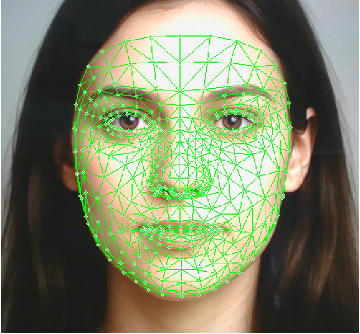
\includegraphics[width=0.5\textwidth]{data/FaceMesh_Mediapipe.png}
    \caption{MediaPipe Face Mesh mit 468 Landmarken, die verschiedene Gesichtsbereiche präzise erfassen}
    \label{fig:mediapipe_face_mesh}
\end{figure}

Die Landmarken sind in semantisch sinnvolle Gruppen unterteilt, was die Erkennung spezifischer Gesichtsmerkmale und -ausdrücke erleichtert. Zur Laufzeit kann die Mesh-Topologie verwendet werden, um die Landmarken in ein dreidimensionales Polygonnetz zu verbinden, was besonders für Augmented-Reality-Anwendungen oder für die 3D-Gesichtsrekonstruktion nützlich ist.

\paragraph{Vortrainierte Lösungen}
MediaPipe bietet vortrainierte Lösungen für gängige Wahrnehmungsaufgaben, darunter:

\begin{itemize}
    \item \textbf{Face Detection:} Schnelle Gesichtserkennung.
    \item \textbf{Face Mesh:} Detaillierte Erkennung von 468 3D-Gesichtslandmarken.
    \item \textbf{Iris Tracking:} Präzise Lokalisierung der Iris.
    \item \textbf{Hands:} Erkennung von Handposen und -landmarken.
    \item \textbf{Pose:} Erkennung von Körperposen und -landmarken.
\end{itemize}

Diese Lösungen sind für verschiedene Plattformen (Android, iOS, Web, Desktop) optimiert und oft in Echtzeit einsetzbar. Sie kapseln die Komplexität der zugrundeliegenden Modelle und bieten einfache APIs.

\paragraph{Einsatz im Projektkontext}
Im Projekt wird MediaPipe für die detaillierte Analyse von Gesichtsmerkmalen genutzt, z.B. für Landmarkenextraktion zur biometrischen Erkennung oder Eye Tracking. Dies ermöglicht präzise und effiziente Erfassung relevanter Merkmale, z.B. für Zutrittskontrollsysteme oder Müdigkeitserkennung. Die Kombination aus schneller Detektion (durch YOLO) und detaillierter Analyse (durch MediaPipe) ergibt eine leistungsfähige Pipeline für Echtzeitanwendungen im Bereich der Gesichtserkennung und -analyse.

\subsubsection{MediaPipe-Architektur und Face Mesh}
MediaPipe ist eine Open-Source-Plattform von Google zur Erstellung plattformübergreifender Pipelines für multimodale Daten. Die Architektur basiert auf modularen Graphen, in denen einzelne Calculatoren Datenvorverarbeitung, ML-Modelle und Nachverarbeitungsschritte verknüpfen.

Das Face Mesh-Modul kombiniert zunächst einen schnellen BlazeFace-Detektor mit einem darauf aufsetzenden Landmarken-Vorhersagemodell und liefert in Echtzeit bis zu 468 3D-Landmarken pro Gesicht. Die Topologie der Landmarken (siehe Abbildung~\ref{fig:mesh_topology}) beschreibt die Kantenverbindungen zwischen den Punkten und ermöglicht eine präzise meshing-Repräsentation.

\begin{figure}[htbp]
    \centering
    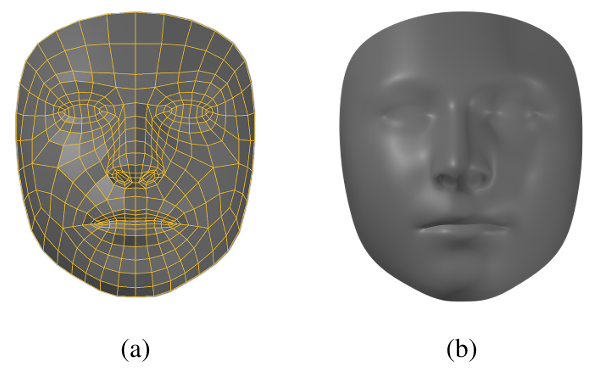
\includegraphics[width=0.8\textwidth]{data/mesh_topology.png}
    \caption{MediaPipe Face Mesh Topologie mit 468 Landmarken und Kantenverbindungen. Quelle: \cite{mediapipe_mesh_topology}}
    \label{fig:mesh_topology}
\end{figure}

\subsection{Funktionsweise von YOLO}

YOLO (\textit{You Only Look Once}) verfolgt einen effizienten Ansatz für die Objekterkennung, der sich durch seine hohe Geschwindigkeit auszeichnet. Anstatt das Bild in mehreren Schritten zu analysieren, betrachtet YOLO das gesamte Bild nur einmal (daher der Name) und sagt alle Objekte gleichzeitig vorher. Man kann sich das wie ein schnelles „Überfliegen“ des Bildes vorstellen.

\begin{figure}[htbp]
    \centering
    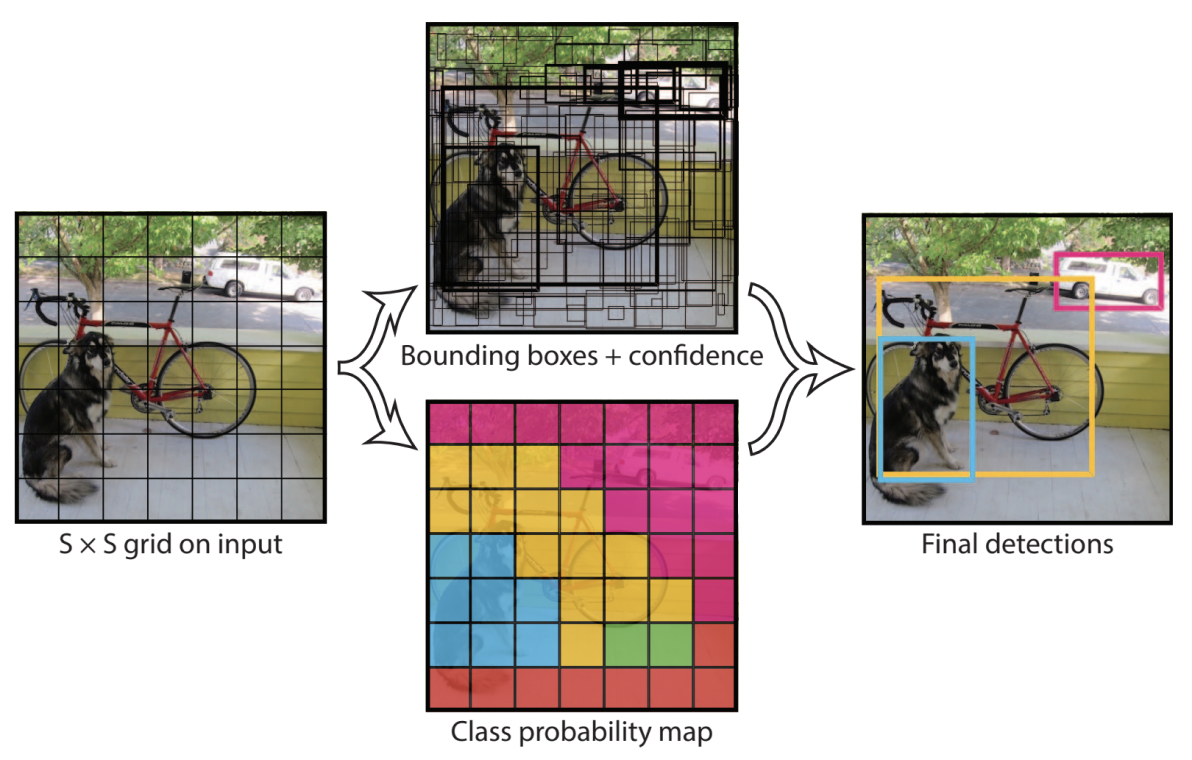
\includegraphics[width=0.8\textwidth]{data/yolo_grid.png}
    \caption{YOLO-Architektur: Das Bild wird in ein Gitter unterteilt, jede Zelle sagt Bounding Boxes und Klassenwahrscheinlichkeiten voraus. Quelle: \cite{yolo_grid}}
    \label{fig:yolo_grid}
\end{figure}

\textbf{Das Gitter (Grid):} \\
Der Kern von YOLO ist die Aufteilung des Eingangsbildes in ein gedachtes Gitter, ähnlich einem Schachbrett (z.B. $13 \times 13$ oder $19 \times 19$ Zellen). Jede dieser Zellen bekommt eine spezielle Aufgabe: Sie ist dafür verantwortlich, Objekte zu erkennen, deren Mittelpunkt genau in diese Zelle fällt.

\textbf{Vorhersagen pro Zelle:} \\
Jede Zelle im Gitter macht mithilfe eines neuronalen Netzes Vorhersagen über mögliche Objekte:
\begin{itemize}
    \item \textbf{Bounding Boxes:} Die Zelle schlägt eine oder mehrere „Boxen“ (Rechtecke) vor, die ein Objekt umschließen könnten. Für jede Box werden Position (x-, y-Koordinaten des Mittelpunkts), Größe (Breite $w$, Höhe $h$) und ein Konfidenzwert vorhergesagt. Dieser Konfidenzwert gibt an, wie sicher sich das Modell ist, dass sich überhaupt ein Objekt in der Box befindet und wie gut die Box passt.
    \item \textbf{Klassenwahrscheinlichkeiten:} Zusätzlich sagt die Zelle voraus, zu welcher Klasse (z.B. „Auto“, „Person“, „Kennzeichen“) ein erkanntes Objekt am wahrscheinlichsten gehört.
\end{itemize}

\textbf{Architektur und Entwicklung:} \\
Das Herzstück ist ein einzelnes Convolutional Neural Network (CNN), das diese Vorhersagen für alle Zellen gleichzeitig generiert. Frühe Versionen nutzten Architekturen wie Darknet. Spätere Versionen (YOLOv3 bis YOLOv8) wurden deutlich komplexer und leistungsfähiger, indem sie z.B. Merkmale aus verschiedenen Ebenen des Netzwerks kombinieren (Feature Pyramid Networks, FPN), um sowohl kleine als auch große Objekte besser zu erkennen. Auch wurden \textit{Anchor Boxes} eingeführt – vordefinierte Box-Formen, die dem Netzwerk helfen, Objekte mit typischen Seitenverhältnissen schneller und genauer zu finden.

\textbf{Aufräumen der Ergebnisse (Non-Max Suppression, NMS):} \\
Da oft mehrere Zellen oder Boxen dasselbe Objekt erkennen, liefert YOLO zunächst viele überlappende Boxen. Um nur die relevanteste Box pro Objekt zu behalten, wird ein „Aufräumschritt“ namens Non-Max Suppression (NMS) durchgeführt. Dabei werden Boxen mit geringer Konfidenz entfernt und von den verbleibenden, überlappenden Boxen wird nur die mit der höchsten Konfidenz behalten, während die anderen verworfen werden.

\textbf{Versionen:} \\
YOLO wird ständig weiterentwickelt. In diesem Projekt kam hauptsächlich YOLOv8 zum Einsatz. Diese Version stellt einen aktuellen Stand der Technik dar und bietet eine gute Balance aus Erkennungsgenauigkeit und hoher Geschwindigkeit, was für die Analyse von Videoströmen vorteilhaft ist. Sie profitiert von den Architekturoptimierungen und Trainingstechniken früherer Versionen und ist oft einfacher zu verwenden. Die Entwicklung schreitet kontinuierlich voran, wie neuere, von Ultralytics dokumentierte Varianten wie YOLOv11 zeigen, was die Dynamik in diesem Bereich unterstreicht.

\subsection{OCR für Texterkennung}

Optical Character Recognition (OCR) bezeichnet den Prozess der Umwandlung von Bildern, die getippten, gedruckten oder handgeschriebenen Text enthalten, in maschinenlesbaren Text. Im Kontext dieses Projekts ist OCR die Schlüsseltechnologie zur Extraktion der Zeichenfolgen aus detektierten Fahrzeugkennzeichen.

\subsubsection{Typische OCR-Pipeline}
Ein OCR-System durchläuft typischerweise mehrere Stufen:

\begin{enumerate}
    \item \textbf{Vorverarbeitung (Preprocessing):} Verbesserung der Bildqualität zur Optimierung der Erkennung. Dies kann Schritte wie Binarisierung (Umwandlung in Schwarz-Weiß), Rauschunterdrückung, Schräglagenkorrektur (Deskewing) und Kontrastanpassung umfassen.

    \item \textbf{Layout-Analyse (oder Segmentierung):} Identifizierung von Textbereichen und deren Struktur. Bei strukturierten Dokumenten wie Kennzeichen kann dies die Segmentierung einzelner Zeichen oder Zeichengruppen umfassen. Bei allgemeineren Texten geht es darum, Absätze, Spalten und Zeilen zu erkennen.

    \item \textbf{Zeichenerkennung (Character Recognition):} Dies ist der Kernschritt, bei dem die segmentierten Zeichen oder Wörter klassifiziert werden. Traditionelle Methoden nutzten Merkmalsextraktion (z.B. topologische Merkmale, Momente) und Klassifikatoren (z.B. SVMs, k-NN). Moderne Ansätze verwenden überwiegend tiefe neuronale Netze, insbesondere CNNs und Recurrent Neural Networks (RNNs), oft in Kombination (CRNN - Convolutional Recurrent Neural Network). RNNs, speziell LSTMs (Long Short-Term Memory), sind gut geeignet, um sequentielle Informationen in Wörtern oder Zeichenketten zu verarbeiten. Attention-Mechanismen können zusätzlich helfen, relevante Bildbereiche für jedes Zeichen zu fokussieren.

    \item \textbf{Nachverarbeitung (Postprocessing):} Korrektur von Erkennungsfehlern unter Verwendung von Sprachmodellen, Wörterbüchern oder kontextuellen Informationen. Bei Kennzeichen kann dies die Überprüfung auf gültige Formate oder die Nutzung von Prüfsummen (falls vorhanden) beinhalten.
\end{enumerate}

\subsubsection{Methoden und Werkzeuge}
Es existieren verschiedene OCR-Engines und Bibliotheken. Eine der bekanntesten Open-Source-Lösungen ist Tesseract OCR, ursprünglich von HP entwickelt und nun von Google weitergeführt. Tesseract verwendet seit Version 4 LSTM-basierte neuronale Netze und bietet eine gute Erkennungsleistung für viele Sprachen und Schriftarten. Daneben gibt es kommerzielle Lösungen und spezialisierte Bibliotheken, die oft für spezifische Anwendungsfälle wie die Kennzeichenerkennung optimiert sind.

\subsubsection{Anwendung bei der Kennzeichenerkennung (ANPR/LPR)}
Automatic Number Plate Recognition (ANPR) oder License Plate Recognition (LPR) ist ein spezialisierter Anwendungsfall von OCR. Die typische Pipeline sieht oft wie folgt aus:

\begin{enumerate}
    \item \textbf{Kennzeichen-Detektion:} Zunächst wird der Bereich des Kennzeichens im Bild lokalisiert. Hierfür eignen sich Objekterkennungsmodelle wie YOLO (siehe Abschnitt 2.2) hervorragend, die darauf trainiert werden, Kennzeichen als Objektklasse zu erkennen.

    \item \textbf{Zeichensegmentierung:} Innerhalb des detektierten Kennzeichenbereichs werden die einzelnen Zeichen isoliert. Dies kann durch traditionelle Bildverarbeitungsalgorithmen (z.B. Konturanalyse, Projektionsprofile) oder durch spezialisierte neuronale Netze erfolgen.

    \item \textbf{Zeichenerkennung:} Jedes segmentierte Zeichen wird durch ein OCR-Modul klassifiziert.
\end{enumerate}

Alternativ können End-to-End-Ansätze verwendet werden, die Detektion und Erkennung in einem einzigen Netzwerk kombinieren oder direkt die gesamte Zeichenkette ohne explizite Segmentierung erkennen.

\subsubsection{Herausforderungen}
Die OCR von Kennzeichen unterliegt spezifischen Herausforderungen wie:
\begin{itemize}
    \item variierenden Lichtverhältnissen (Tag/Nacht, Schatten, Blendung),
    \item unterschiedlichen Kameraperspektiven und -abständen,
    \item Verschmutzung oder Beschädigung der Kennzeichen,
    \item verschiedenen Kennzeichenlayouts und Schriftarten (je nach Land/Region),
    \item Bewegungsunschärfe
\end{itemize}

Die Robustheit des OCR-Systems gegenüber diesen Faktoren ist entscheidend für die praktische Anwendbarkeit.

\subsection{Gesichtserkennung mit neuronalen Netzen}

Die Gesichtserkennung ist ein Spezialfall der Objekterkennung und der biometrischen Identifikation, die in den letzten Jahren durch den Einsatz neuronaler Netze erhebliche Fortschritte erzielt hat. Sie umfasst typischerweise mehrere Schritte: Gesichtsdetektion, Vorverarbeitung, Merkmalsextraktion und Vergleich oder Klassifikation.

\subsubsection{Technologien im Detail}

\paragraph{Gesichtsdetektion} 
Wie in Abschnitt 2.1 und 2.2 beschrieben, können Modelle wie YOLO hierfür eingesetzt werden. Alternativ nutzen viele Frameworks dedizierte, oft schnellere Detektoren (z.B. basierend auf SSD oder spezialisierten Architekturen).

\paragraph{Landmarken-Detektion} 
Frameworks wie Google's MediaPipe bieten spezialisierte Modelle zur Detektion von hunderten Gesichtslandmarken in Echtzeit (z.B. das Face Mesh mit 468 3D-Landmarken). Diese Landmarken sind nützlich für die Gesichtsausrichtung, Mimik- und Augenbewegungsanalyse (z.B. Eye Tracking) sowie die Extraktion biometrischer Merkmale. Sie können als Merkmalsvektor dienen, wobei für die Identifikation meist Embeddings aus tieferen CNNs verwendet werden.

\paragraph{Biometrische Identifikation und Verifikation}
In der biometrischen Gesichtserkennung werden individuelle physiologische Gesichtsmerkmale wie Gesichtsform, Abstand der Augen, Ausprägung der Nasen- und Mundpartie sowie weitere geometrische Beziehungen genutzt, um Personen zu identifizieren oder zu verifizieren. Diese Merkmale werden in mathematischen Repräsentationen (Gesichts-Embeddings) kodiert, die für jede Person einzigartig sind. Der Vorteil biometrischer Systeme ist, dass sie auf inhärente Eigenschaften zurückgreifen, die nicht wie Passwörter vergessen oder wie Ausweise verloren werden können. Neurale Netzwerke haben dabei entscheidende Verbesserungen in der Zuverlässigkeit und Robustheit gebracht, insbesondere gegenüber Variationen in Beleuchtung, Gesichtsausdruck und Alterung.

\paragraph{Embedding-Generierung} 
Bibliotheken wie \texttt{face\_recognition} (basierend auf dlib) vereinfachen die Implementierung von Gesichtserkennungspipelines. Sie kapseln Detektion, Landmarken-Findung und Embedding-Generierung mithilfe vortrainierter Modelle (z.B. ResNet-basiert) und liefern 128-dimensionale Embeddings für den Vergleich. Diese hochdimensionalen Vektoren kodieren die unverwechselbaren Merkmale eines Gesichts in einem mathematischen Raum, in dem die euklidische Distanz zwischen Embeddings als Ähnlichkeitsmaß verwendet wird. Für die Verifikation wird typischerweise ein Schwellenwert festgelegt – liegt die Distanz unter diesem Wert, gilt das Gesicht als verifiziert.

\paragraph{Gesichtsliveness-Erkennung}
Um Sicherheitsrisiken durch Präsentationsangriffe (z.B. Verwendung von Fotos oder Videos) zu minimieren, implementieren moderne biometrische Systeme Liveness-Erkennungstechniken. Diese können aktive Methoden (Aufforderung zu Bewegungen wie Blinzeln oder Kopfdrehen) oder passive Methoden (Analyse von Mikrotexturen der Haut, Erfassung unwillkürlicher Bewegungen oder Erkennung von Reflexionseigenschaften) umfassen. Moderne KI-Systeme kombinieren diese Ansätze mit tiefen neuronalen Netzen, die Echtzeitanalysen der Bilddaten ermöglichen und die Sicherheit biometrischer Anwendungen erhöhen.
